\section{SURF}
SpeededUp Robust Features (SURF), introduceret af Bay et. al \cite{SURF} og er ligesom SIFT en samlet metode, bestående af en detektor og en deskriptor, der lokalisere og beskriver blobs af forskellige størrelser.
\subsection{Determinant of Hessian}
Determinant of Hessian eller \textit{DoH}: $\textbf{det}\mathcal{H}L$ , udgør feature detektoren i
SURF. DoH er baseret på Hessian matricen, som udregnes for hvert punkt $p=(x,y)$ i et billede:
\begin{equation}
\mathcal{H}(p, \sigma) = 
 \begin{bmatrix}
 	L_{xx}(p, \sigma) & L_{xy}(p, \sigma) \\
 	L_{xy}(p, \sigma) & L_{yy}(p, \sigma) 
 \end{bmatrix}
 \label{hessianmatrix}
\end{equation}
hvor $\sigma$ svarer til skalaen og $L_{xy} $, $L_{yy}$ og $L_{xx}$\eqref{lxx}, er den Gaussiske funktionen, partielt differentieret ifht. $xy$, $yy$ og $xx$.
\begin{equation}
L_{xx}(x, \sigma) = (\frac{\partial^2 }{\partial x^2 } G(x,y,\sigma)) * I
\label{lxx}
\end{equation}
Bay et.al anvender approkismerede, vægtede box filtrer $D_{xx}$, $D_{yy}$ og $D_{xy}$, der ved brug af integralbilleder nedsætter antallet af beregninger drastisk. Disse filtrer består udelukkende af værdier af -2,-1,0 eller 1. I implementeringen er disse boxfiltrer ikke anvendt, og er derved udregnet som i \eqref{lxx}, figur \ref{fig:lxxlyylxy} viser en illustration af de anvendte filtre.
\begin{figure}[H]
    \centering
    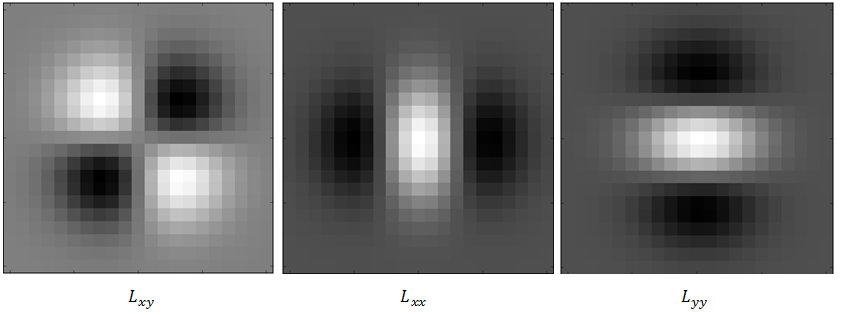
\includegraphics[width=0.75\textwidth]{fig/31.png}
     \vspace{-0.5em}
    \begin{center}    
       \caption{\textcolor{gray}{\footnotesize \textit{ }}}
    \label{fig:lxxlyylxy}
     \end{center}
     \vspace{-2.5em}
  \end{figure} \noindent
I metoden oprettes skalarummet ved iterativt at forøge størrelsen af filtrene, med $\sigma=1.2$, fremfor at forøge størrelsen af $\sigma$. For hver oktav, eksisterer, i denne implementering, fire billeder, foldet med fire forskellige filterstørrelser. For hver oktav, bruges nr. to filterstørrelse, fra forrige oktav til starten af den næste oktav, og størrelsen imellem filtre, fordobles fra forrige oktav, som vist i tabel \ref{fig:secderivfiltersize}. Her skal det bemærkes, at de andenafledte filtre, skal have dobbelt størrelse, af de førsteafledte, som er vist i tabel \ref{fig:firstderivfiltersize}
\begin{figure}[H]
    \centering
    \begin{center}    
    \begin{tabular}{ | l | l | l | l | l |}
    \hline
    oktav & filter str 1 & filter str 2 & filter str 3 & filter str 4 \\ \hline
    1 & 9 & 15 & 21 & 27 \\ \hline
  	2 & 15 & 27 & 39 & 51 \\ \hline
  	3 & 27 & 51 & 75 & 99 \\ \hline
  	4 & 51 & 99 & 147 & 195 \\ \hline
    \end{tabular}       
    \caption{\textcolor{gray}{\footnotesize \textit{Fire forskellige oktaver, og filterstørrelse, for et andenafledt filter}}}
    \label{fig:secderivfiltersize}
     \end{center}
     \vspace{-2.5em}
  \end{figure} \noindent
For hvert punkt i billederne opstilles Hessian matricen, hvorefter determinten udregnes for alle punkter i billederne. Bay et.al. udregner determinanten ved:
\begin{equation}
\textbf{det}\mathcal{H}_{approksimeret} = D_{xx}D_{yy}-wD_{xy}^2
\label{deerminantofhessian}
\end{equation}
, hvor $w$ er en vægt, tilføjet, for at balancere de approksimerede filtre og boks filtrene. Da denne implementering ikke anvender boks filtrer udregnes determinanten som:
\begin{equation}
\textbf{det}\mathcal{H} = L_{xx}L_{yy}-L_{xy}^2
\label{deerminantofhessian}
\end{equation}
Determinant of Hessian reagere på mørke og lyse blobs, ved positive svar. Derfor udvælges et lokalt maxima af et $3\times3\times3$ område af determinantbillederne, som vist på figur \ref{fig:difference}. Dette udføres for alle oktaver. Herefter udvælges korrekt subpixel placering, hvilket er en metode introduceret af David Lowe, også beskrevet i SIFT. Igen udføres dette skridt ved at fjerne punkter ikke lokaliseret tæt nok på ekstremaer og svage ekstremaer.
\subsection*{Algoritme}
\begin{enumerate}
\item {Hessian matricen opstilles for alle punkter i skalabillederne som:
$$
\mathcal{H} = 
 \begin{bmatrix}
 	L_{xx} & L_{xy} \\
 	L_{xy} & L_{yy} 
 \end{bmatrix} $$
}
\item Determinantbilleder opstilles, ved at udregne determinanten af Hessian matricen for alle punkter i alle billeder ved:
$$
\textbf{det}\mathcal{H} = L_{xx}L_{yy}-L_{xy}^2
$$
\item Lokale maxima udvælges, af hvert $3\times3\times3$ område af billeder på samme oktav.
\item Accurate keypoint localisation, bruges til at fjerne dårligt lokaliserede punkter.
\end{enumerate}
\subsection{SURF orientering}
SURF gør brug af Haar-wavelet filter, når en orientering for interessepunkter skal bestemmes og i deskriptoren. Haar-wavelet er et boksfilter, med størrelse ($N\times N$), hvor halvdelen af alle indgangene er 1 og den anden halvdel er -1. Filtret i figur \ref{fig:haarwavelet} kaldes $dx$ (venstre) og $dy$ (højre).
\begin{figure}[H]
    \centering
    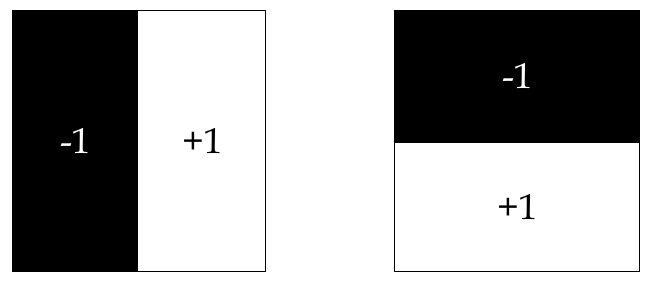
\includegraphics[width=0.55\textwidth]{fig/haarwavelet.png}
     \vspace{-1em}
    \begin{center}    
       \caption{\textcolor{gray}{\footnotesize \textit{ }}}
    \label{fig:haarwavelet}
     \end{center}
     \vspace{-2.5em}
  \end{figure} \noindent
$dx$ og $dy$ beregnes i en cirkel omkring interessepunktet, som udgør et dataindsamlingsvindue $D_x$ og $D_y$, med radius $6\sigma$, og en afstand mellem punkterne, på $\sigma$. $D_x$ og $D_y$ foldes med en Gausskerne, hvor $\sigma_{Gauss} = 2.5\sigma$.
\begin{figure}[H]
    \centering
    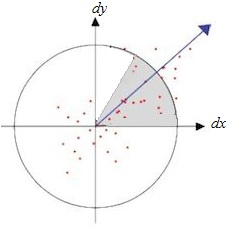
\includegraphics[width=0.2\textwidth]{fig/surforientation.jpg}
     \vspace{-1em}
    \begin{center}    
       \caption{\textcolor{gray}{\footnotesize \textit{ }}}
    \label{fig:surforientation}
     \end{center}
     \vspace{-2.5em}
  \end{figure} \noindent
$D_x$ og $D_y$ udgør et sæt af punkter, der kan plottes som illustreret figur \ref{fig:surforientation}. Hver punkt udgør en vektor. Et vindue på $60^{\circ}$, summerer alle vektorene, der ligger indenfor dets rækkevidde (grå markering). Af de summerede vektorer udgør den længste vektor, punktets orientering. Dette er illustreret på figur \ref{fig:surforientation}. Der er her taget en beslutning om, at slidingvinduet udregner summen af vektorer, indenfor seks positioner ($0^{\circ}-60^{\circ}$, $60^{\circ}-120^{\circ}$,..., $300^{\circ}-360^{\circ}$).
\\
Ovenstående udregning tildeler alle interessepunkter en orientering $\theta$.
\subsubsection*{Algoritme: SURF Orientering}
\begin{tabbing}
Input\quad \= : \= Billede $I$\\
$\text{ }$ \> : \>  Interessepunkter $p \in (x, y)$ \\
Output \text{ } \> : \> Interessepunkter med orientering $p \in (x, y, \theta)$
\end{tabbing}
\begin{enumerate}
\item Orienteringen på punktet findes, ved at beregne $D_x$, $D_y$ i et cirkulært område, med radius $6\sigma$, og afstand $\sigma$, mellem punkterne. 
\item $D_x$, $D_y$ foldes med en Gausskerne, med $\sigma_{Gauss} = 2.5\sigma $.
\item Den længste vektor, af summerede vektorer, der ligger indenfor $60^{\circ}$, bruges til at tildele orientering $\theta$ til interessepunktet.
\end{enumerate}
SURF deskriptoren producerer features, der består af 64 indgange. Som beskrevet af Tuytelaars et. al \cite{SURF}, er tilfældet ofte, at der ikke er brug for rotationsinvarians. En variant af SURF, der ikke er rotationsinvariant, kaldes Upright-SURF (U-SURF). Tuytelaars et. al garanterer dog rotationsinvarians i U-SURF, i op til $\pm 15^{\circ}$. SURF er implementeret, fremfor U-SURF, da enkelte af billederne har stor grad (ca. $15^{\circ}$) af rotation. Rotationen forekommer i billeder, der er taget lige efter, at dronen har vendt og kan ses på figur <[???]>.
\\
\\
SURF deskriptoren indsamler data omkring interssepunktet, med et dataindsamlingvindue der har størrelse $20 \sigma$. Vinduet skal orienters, ifht. den $\theta$ værdi, der er udregnet. Dette gøres ved, at hele billedet vendes, ved brug af ligning \eqref{rotaionmatrix}, og der dannes et integralbillede ud fra det roterede billede <(Dette skridt er omkostningsfuldt, og der vil senere blive diskuteret optimeringer)>.
\\
\\
Dataindsamlingsvinduet er nu roteret og centreret omkring interessepunktet. Herefter skal vinduet deles op i 4x4 regioner, hver bestående af 5x5 punkter, der har ens afstand mellem sig - her er ikke blevet lavet subpixel-interpolation, så hvis $\frac{20\sigma}{4}$ ikke er deleligt med 5, bliver der rundet ned.
\\
\\
Herefter skal $dx$ og $dy$ udregnes. Haar-wavelet skal udregnes for alle punkterne i vinduet. Størrelsen på Haar-wavelet filteret, er $2\sigma$. Vinduet skal smoothes med et Gaussfilter, hvor $\sigma_{Gauss} = 3.3\sigma_{point}$.
\\
\\
For hver af de 16 4x4 regioner, udregnes: 
\begin{equation}
v_i = \sum d_x, \sum d_y, \sum |d_y|, \sum |d_y|
\label{surffeature}
\end{equation}
hvor $v_i$ er en $(4x1)$ matrix, for region nr. $i$, hvor hver region er nummeret i læseretningen. Der dannes en feature vektor $F$, ved at sammensætte alle $v_i$: $F = [v_1^T, v_2^T,..., v_16^T]^T$. Dette giver en $16 \cdot 4 = 64$ indgange stor vektor. Slutteligt, laves vektoren til en enhedsvektor.
\subsubsection*{Algoritme: SURF Deskriptor}
\begin{tabbing}
Input\quad \= : \= Billede $I$\\
$\text{ }$ \> : \> Punkter $p \in (x, y, \theta)$ \\
Output \text{ } \> : \> En feature vektor $F$, for hver punkt $p$.
\end{tabbing}
\begin{enumerate}
\item Et dataindsamlingsvindue roteret ifht. $\theta$, beregnet som \eqref{rotaionmatrix} med størrelse $20\sigma$ indsamler punkter, der er har afstand $\sigma$ mellem hinanden.
\item Haar-wavelet responset, $dx$, $dy$ udregnes for de indsamlede punkter, med en filterstørrelse på $2\sigma$, og $dx, dy$ foldes med Gauss, hvor $\sigma_{Gauss} = 3.3\sigma$.
\item For hver af de 4x4 regioner, udregnes \eqref{surffeature}. Dette sættes sammen til en vektor, der vil have 64 indgange.
\end{enumerate}